% !TEX root = ../main.tex

\clearpage
% Source PDF page 6.
\section{第三章\quad 奶蛙的诞生与奶蛙发展史}

\subsection{一、奶蛙的诞生}

奶蛙的出处一直纷争不断。大家都知道奶蛙是由奶龙通过 AI 转换形象而来的，但是究竟是谁率先做出了初版的奶蛙形象？这个问题直到 2026 年 8 月 5 日才被以 B 站 up 主看仙碎为首的一大批奶蛙爱好者解决（视频号 BV1ndMk65EwM）。

2024 年 10 月 2 日，星野 AI 用户纲手【百豪】创建了世界上第一个带有明显奶蛙特征的奶龙智能体。星野 AI 会把用户输入的图片 AI 化重新处理之后作为智能体的封面，而正是在误打误撞的情况下，奶蛙的原型图片诞生了。奶蛙的生日被普遍取为 10 月 2 日这一天。~(见\figref{fig:03-1})

% !TEX root = ../../main.tex
\begin{figure}[H]
  \centering
  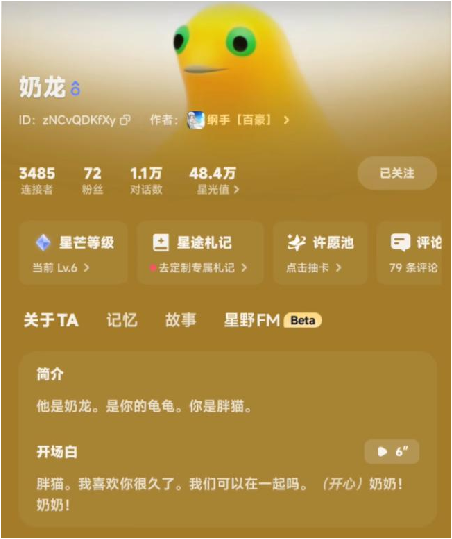
\includegraphics[width=184.25bp,height=0.76\textheight,keepaspectratio]{figures/chapter03/figure03_1.pdf}
  \renewcommand{\thefigure}{3.1}
  \caption{纲手【百豪】创建的奶龙智能体，可看到最初版奶蛙的图片}
  \label{fig:03-1}
\end{figure}


\subsection{二、奶蛙发展史}

至此，奶蛙开始作为奶龙的一个变种出现。凭借着诡异的身体形态，奶蛙很快受到了大量关注。~(见\figref{fig:03-2})

% !TEX root = ../../main.tex
\begin{figure}[H]
  \centering
  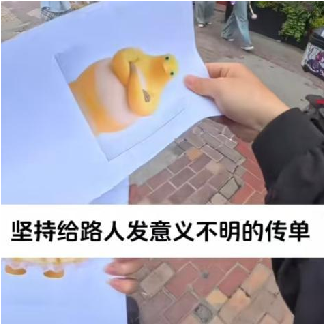
\includegraphics[width=132.74bp,height=0.76\textheight,keepaspectratio]{figures/chapter03/figure03_2.pdf}
  \renewcommand{\thefigure}{3.2}
  \caption{奶蛙的图片被大量用作意义不明传单挑战}
  \label{fig:03-2}
\end{figure}


然而，目前的奶蛙仅仅是奶龙的附庸，缺少自己的独到特色。

而最好的特色，无疑就是一个充满魔性的声音。

